%%%%%%%%%%%%%%%%%%%%%%%%%%%%%%%%%%%%%%%%%%%%%%%%%%%%%%%%%%%%%%%%%%%%%%%%%%%%%%%%
% Building interactive applications with ETS
%
% Author: Enthought, Inc. Mumbai, India
% Copyright (c) 2012 Enthought Inc., Mumbai India
%%%%%%%%%%%%%%%%%%%%%%%%%%%%%%%%%%%%%%%%%%%%%%%%%%%%%%%%%%%%%%%%%%%%%%%%%%%%%%%%

\documentclass[14pt,compress]{beamer}

% Modified from: generic-ornate-15min-45min.de.tex
\mode<presentation>
{
  \usetheme{Warsaw}
  \useoutertheme{infolines}
  \setbeamercovered{transparent}
}

\usepackage[english]{babel}
\usepackage[latin1]{inputenc}
%\usepackage{times}
\usepackage[T1]{fontenc}
\usepackage{pgf}
\usepackage{amsmath}

% Taken from Fernando's slides.
\usepackage{ae,aecompl}
\usepackage{mathpazo,courier,euler}
\usepackage[scaled=.95]{helvet}

\definecolor{darkgreen}{rgb}{0,0.5,0}

\usepackage{listings}
\lstset{language=Python,
    basicstyle=\ttfamily\bfseries,
    commentstyle=\color{red}\itshape,
  stringstyle=\color{darkgreen},
  showstringspaces=false,
  keywordstyle=\color{blue}\bfseries}

%%%%%%%%%%%%%%%%%%%%%%%%%%%%%%%%%%%%%%%%%%%%%%%%%%%%%%%%%%%%%%%%%%%%%%
% Macros
\setbeamercolor{emphbar}{bg=blue!20, fg=black}
\newcommand{\emphbar}[1]
{\begin{beamercolorbox}[rounded=true]{emphbar} 
      {#1}
 \end{beamercolorbox}
}
\newcounter{time}
\setcounter{time}{0}
\newcommand{\inctime}[1]{\addtocounter{time}{#1}{\tiny \thetime\ m}}

\newcommand{\typ}[1]{\lstinline{#1}}
\newcommand{\myemph}[1]{\structure{\emph{#1}}}
\newcommand{\PythonCode}[1]{\lstinline{#1}}

\newcommand{\kwrd}[1]{ \texttt{\textbf{\color{blue}{#1}}}  }

\newcommand\BackgroundPicture[1]{%
  \setbeamertemplate{background}{%
      \parbox[c][\paperheight]{\paperwidth}{%
      \vfill \hfill
        \pgfimage[width=1.0\paperwidth,height=1.0\paperheight,interpolate=true]{#1}
 \hfill \vfill
}}}

% For non-wide pictures, set the width so that the height scales
% appropriately.
\newcommand\BackgroundPictureWidth[1]{%
  \setbeamertemplate{background}{%
      \parbox[c][\paperheight]{\paperwidth}{%
      \vfill \hfill
        \pgfimage[width=1.0\paperwidth,interpolate=true]{#1}
 \hfill \vfill
}}}


% For shorter pictures, set the height so that the width scales
% appropriately.
\newcommand\BackgroundPictureHeight[1]{%
  \setbeamertemplate{background}{%
      \parbox[c][\paperheight]{\paperwidth}{%
      \vfill \hfill
        \pgfimage[height=1.0\paperheight,interpolate=true]{#1}
 \hfill \vfill
}}}


%%% This is from Fernando's setup.
% \usepackage{color}
% \definecolor{orange}{cmyk}{0,0.4,0.8,0.2}
% % Use and configure listings package for nicely formatted code
% \usepackage{listings}
% \lstset{
%    language=Python,
%    basicstyle=\small\ttfamily,
%    commentstyle=\ttfamily\color{blue},
%    stringstyle=\ttfamily\color{orange},
%    showstringspaces=false,
%    breaklines=true,
%    postbreak = \space\dots
% }

%%%%%%%%%%%%%%%%%%%%%%%%%%%%%%%%%%%%%%%%%%%%%%%%%%%%%%%%%%%%%%%%%%%%%%
% Title page
\title[ETS]{Building interactive applications with ETS}

\author[Prabhu and Pankaj] {Prabhu Ramachandran and Pankaj Pandey}

\institute[Enthought] {\large \pgfimage[height=3em]{enthought-logo_lg}
}
\date[] {
\small
PyCon India, Bangalore\\
September 28, 2012
}
%%%%%%%%%%%%%%%%%%%%%%%%%%%%%%%%%%%%%%%%%%%%%%%%%%%%%%%%%%%%%%%%%%%%%%

\pgfdeclareimage[height=0.75cm]{enthought-logo}{enthought-logo}
\logo{\pgfuseimage{enthought-logo}}


%% Delete this, if you do not want the table of contents to pop up at
%% the beginning of each subsection:
\AtBeginSubsection[]
{
  \begin{frame}<beamer>
    \frametitle{Outline}
    \tableofcontents[currentsection,currentsubsection]
  \end{frame}
}

\AtBeginSection[]
{
  \begin{frame}<beamer>
    \frametitle{Outline}
    \tableofcontents[currentsection,currentsubsection]
  \end{frame}
}

% If you wish to uncover everything in a step-wise fashion, uncomment
% the following command: 
%\beamerdefaultoverlayspecification{<+->}

%%\includeonlyframes{current,current1,current2,current3,current4,current5,current6}

%%%%%%%%%%%%%%%%%%%%%%%%%%%%%%%%%%%%%%%%%%%%%%%%%%%%%%%%%%%%%%%%%%%%%%
% DOCUMENT STARTS
\begin{document}

\begin{frame}
  \maketitle
\end{frame}


\begin{frame}
  \frametitle{About the Tutorial}
  \begin{block}{Intended Audience}
  \begin{itemize}
    \item Use Python to build interactive desktop applications
  \end{itemize}
  \end{block}  

  \begin{block}{Goal: Successful participants will be able to}
    \begin{itemize}
      \item Start using Enthought Tool Suite (ETS) to build non-trivial applications

    \end{itemize}
  \end{block}
\end{frame}

%%%%%%%%%%%%%%%%%%%%%%%%%%%%%%%%%%%%%%%%%%%%%%%%%%%%%%%%%%%%%%%%%%%%%%%%%%%%%%%
\section{Introduction}

\begin{frame}
  \frametitle{}
  \begin{center}
    \pgfimage[height=0.9\paperheight]{images/ODEApp}  
  \end{center}
\end{frame}

\begin{frame}
  \frametitle{Approach}
  \begin{itemize}
      \item A graphical explorer for ODEs \alert{from the ground up}
  \item Support arbitrary 2 and 3 dimensional systems
  \item Using ETS
 \end{itemize}
\end{frame}

\begin{frame}
  \frametitle{Why?}
  \begin{itemize}
  \item Something interesting and concrete
  \item Same ideas extend to other situations
 \end{itemize}
\end{frame}

\subsection{ODE 101}


\begin{frame}
  \frametitle{ODE 101}
  \begin{itemize}
    \item Used to model many systems
        \begin{itemize}
            \item Physics, astronomy
            \item Geology (weather modeling)
            \item Chemistry (reactions)
            \item Biology
            \item Ecology/population modeling
            \item Economics (stock trends, interest rates etc.)
        \end{itemize}
    \item Rich behavior
    \item Numerical solution: \typ{scipy}
 \end{itemize}
\end{frame}

\begin{frame}
  \frametitle{Simple equation}
\begin{align}
    \frac{dx}{dt} = f(x, t)
\end{align}
\emph{x} can be a vector with many components.
\end{frame}


\begin{frame}[fragile]
\frametitle{Solving ODEs using SciPy}
\begin{itemize}
\item Consider the spread of an epidemic in a population
\item $\frac{dy}{dt} = ky(L-y)$ gives the spread of the disease
\item $L$ is the total population.
\item Use $L = 2.5E5, k = 3E-5, y(0) = 250$
\item Define a function as below
\end{itemize}
\small
\begin{lstlisting}
In []: from scipy.integrate import odeint
In []: def epid(y, t):
  ....     k = 3.0e-5
  ....     L = 2.5e5
  ....     return k*y*(L-y)
  ....
\end{lstlisting}
\end{frame}

\begin{frame}[fragile]
\frametitle{Solving ODEs using SciPy \ldots}
\begin{lstlisting}
In []: t = linspace(0, 12, 61)

In []: y = odeint(epid, 250, t)

In []: plot(t, y)
\end{lstlisting}
%Insert Plot
\end{frame}

\begin{frame}[fragile]
\frametitle{Result}
\begin{center}
    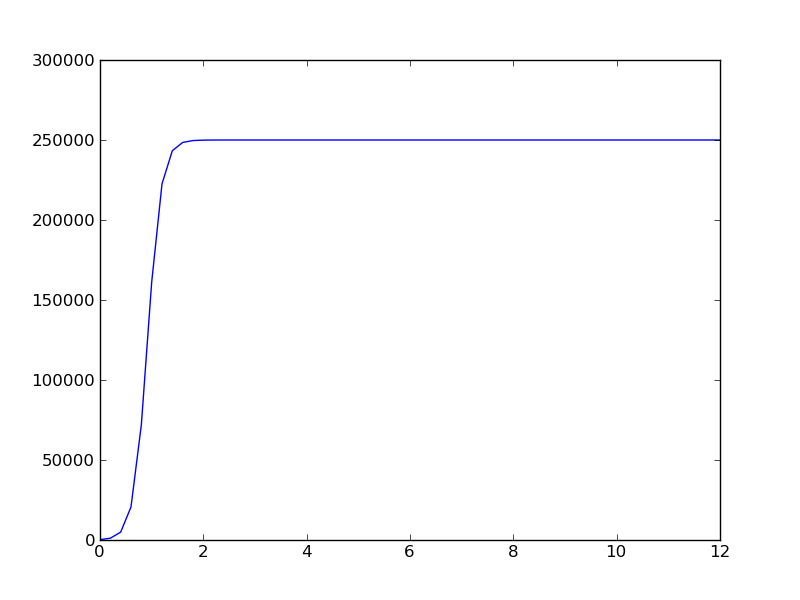
\includegraphics[height=2in, interpolate=true]{images/population_ode}
\end{center}
\end{frame}

% \begin{frame}[fragile]
% \frametitle{ODEs - Simple Pendulum}
% We shall use the simple ODE of a simple pendulum. 
% \begin{equation*}
% \ddot{\theta} = -\frac{g}{L}sin(\theta)
% \end{equation*}
% \begin{itemize}
% \item This equation can be written as a system of two first order ODEs
% \end{itemize}
% \begin{align}
% \dot{\theta} &= \omega \\
% \dot{\omega} &= -\frac{g}{L}sin(\theta) \\
%  \text{At}\ t &= 0 : \nonumber \\
%  \theta = \theta_0(10^o)\quad & \&\quad  \omega = 0\ (Initial\ values)\nonumber 
% \end{align}
% \end{frame}
% 
% \begin{frame}[fragile]
% \frametitle{ODEs - Simple Pendulum \ldots}
% \begin{itemize}
% \item Use \typ{odeint} to do the integration
% \end{itemize}
% \begin{lstlisting}
% In []: def pend_int(initial, t):
%   ....     theta = initial[0]
%   ....     omega = initial[1]
%   ....     g = 9.81
%   ....     L = 0.2
%   ....     F=[omega, -(g/L)*sin(theta)]
%   ....     return F
%   ....
% \end{lstlisting}
% \end{frame}
% 
% \begin{frame}[fragile]
% \frametitle{ODEs - Simple Pendulum \ldots}
% \begin{itemize}
% \item \typ{t} is the time variable \\ 
% \item \typ{initial} has the initial values
% \end{itemize}
% \begin{lstlisting}
% In []: t = linspace(0, 20, 101)
% In []: initial = [10*2*pi/360, 0]
% \end{lstlisting} 
% \end{frame}
% 
% \begin{frame}[fragile]
% \frametitle{ODEs - Simple Pendulum \ldots}
% %%\begin{small}
% \typ{In []: from scipy.integrate import odeint}
% %%\end{small}
% \begin{lstlisting}
% In []: pend_sol = odeint(pend_int, 
%                          initial,t)
% \end{lstlisting}
% \end{frame}
% 
% \begin{frame}[fragile]
% \frametitle{Result}
% \begin{center}
%     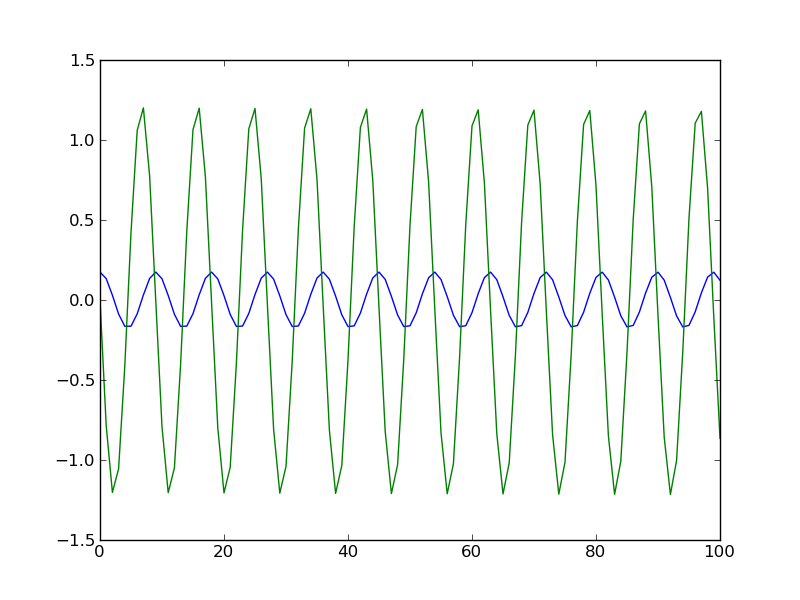
\includegraphics[height=2in, interpolate=true]{images/pendulum_ode}
% \end{center}
%   \inctime{10}
% \end{frame}

\begin{frame}[plain]
    \frametitle{Lorenz equation example}
    \begin{eqnarray*}
        \frac{d x}{dt} &=& s (y-x)\\
        \frac{d y}{d t} &=& rx -y -xz\\
        \frac{d z}{d t} &=& xy - bz\\
    \end{eqnarray*}
    \begin{itemize}
        \item Specifies the evolution of the system
        \item Think: Velocity of a particle in 3D
        \item Lets trace its path
    \end{itemize}
\end{frame}

\begin{frame}[plain,fragile]
    \frametitle{Solution}
\small
  \begin{lstlisting}
import numpy as np
from scipy.integrate import odeint
def lorenz(r, t s=10.,r=28., b=8./3.):
    x, y, z = r
    u = s*(y-x)
    v = r*x -y - x*z
    w = x*y - b*z
    return np.array([u, v, w])

start = (10., 50., 50.)
t = np.linspace(0., 50., 2000)
r = odeint(lorenz, start, t)
x, y, z = r[:,0], r[:,1], r[:,2]

mlab.plot3d(x, y, z, t, 
from mayavi import mlab
                tube_radius=None)
\end{lstlisting}
\end{frame}

\BackgroundPicture{images/lorenz_traj}
\begin{frame}[plain]
\end{frame}
\BackgroundPicture{images/blank}

\begin{frame}
  \frametitle{Now what?}
  \begin{itemize}
      \item An application to explore these
      \item Use cases
          \begin{itemize}
              \item Interactive exploration
              \item Change the equations on UI
              \item See output immediately
              \item Standard equations (fully setup)
          \end{itemize}
 \end{itemize}
\end{frame}


\begin{frame}
  \frametitle{ETS: Enthought Tool Suite}
  \begin{itemize}
    \item Traits: Object Models
    \item TraitsUI: Views for Objects having Traits
    \item Chaco: 2D Visualizations
    \item Mayavi: 3D Visualizations
    \item Envisage: Application Framework
    \vspace*{0.5in}
    \item Miscellaneous libraries
  \end{itemize}
\end{frame}



%%%%%%%%%%%%%%%%%%%%%%%%%%%%%%%%%%%%%%%%%%%%%%%%%%%%%%%%%%%%%%%%%%%%%%%%%%%%%%%
\section{Traits}

\begin{frame}
  \frametitle{Introduction to Traits}
  \begin{itemize}
    \item  \alert{trait}: Python object attribute with additional characteristics
    \vspace*{2em}

    \item \url{http://code.enthought.com/projects/traits}
    \item \url{http://github.enthought.com/traits/tutorials}

  \end{itemize}
\end{frame}

\begin{frame}
  \frametitle{Trait features}
  \begin{itemize}
    \item Initialization: default value
    \item Validation: strongly typed
    \item Delegation: value delegation
    \item Notification: events
    \item Visualization: MVC, automatic GUI!
  \end{itemize}
\end{frame}

\begin{frame}[fragile,plain]
  \frametitle{Traits Example}
\vspace*{-16pt}
\footnotesize
\begin{lstlisting}
from traits.api import (Delegate, HasTraits, 
    Instance, Int, Str)

class Parent(HasTraits):
    # INITIALIZATION: 'last_name' initialized to ''
    last_name = Str('') 
\end{lstlisting}
\pause
\begin{lstlisting}
class Child(HasTraits):
    age = Int
    # VALIDATION: 'father' must be Parent instance
    father = Instance(Parent)
    # DELEGATION: 'last_name' delegated to father's 
    last_name = Delegate('father') 
    # NOTIFICATION: Method called when 'age' changes
    def _age_changed(self, old, new): 
        print 'Age changed from %s to %s ' % (old, new)
\end{lstlisting}
\end{frame}

\begin{frame}[fragile,plain]
  \frametitle{Traits Example}
\vspace*{-6pt}
\small
\begin{lstlisting}
In []: joe = Parent()
In []: joe.last_name = 'Johnson'
In []: moe = Child()
In []: moe.father = joe

In []: moe.last_name # Delegation
Out[]: "Johnson"

In []: moe.age = 10 # Notification
Age changed from 0 to 10

In []: moe.configure_traits() # Visualization
\end{lstlisting}
\inctime{10}
\end{frame}


\begin{frame}[fragile,plain]
    \frametitle{Predefined Trait Types}
    \vspace*{-6pt}
    \small
    \begin{itemize}
        \item Standard: \typ{Bool, Int, Float, Str, Tuple, List, Dict}
        \item Constrained: \typ{Range, Regex, Expression, ReadOnly}
        \item Special: \typ{Either, Enum, Array, File, Color, Font}
        \item Generic: \typ{Instance, Any, Callable}
        \item ...
        \item Custom traits: 2D/3D plots etc.
    \end{itemize}
\end{frame}

\begin{frame}[fragile,plain]
    \frametitle{Trait Change Notifications}
    \vspace*{-6pt}
    \small
    \begin{itemize}
        \item Static: \typ{def _<trait_name>_changed()}
        \item Decorator: \typ{@on_trait_change('extended.trait[].name')}
        \item Dynamic:
    \end{itemize}
\begin{lstlisting}
obj.on_trait_change(handler, 
                    ['extended.trait[].name'])
\end{lstlisting}
\end{frame}

\begin{frame}[fragile,plain]
  \frametitle{Notification Example}
\vspace*{-8pt}
\footnotesize
\begin{lstlisting}
from traits.api import (Delegate, HasTraits, 
    Instance, Int, Str, on_trait_change)
class Parent(HasTraits):
    last_name = Str('') 
class Child(HasTraits):
    age = Int
    father = Instance(Parent)
\end{lstlisting}
\pause
\begin{lstlisting}
    def _age_changed(self, old, new):
        print 'Age changed from %s to %s ' % (old, new)

    @on_trait_change('father.last_name')
    def _dad_name_updated(self):
        print self.father.last_name

def handler(obj, name, old, new):
    print obj, name, old, new

c = Child(father=Parent(last_name='Ram'))
c.on_trait_change(handler, ['father', 'age'])

\end{lstlisting}
\end{frame}


\begin{frame}
  \frametitle{Designing the ODE explorer app}
  \Large
\begin{center}
    \pause
    \myemph{Think!}

    \vspace*{1in}
    Focus on the object model
\end{center}
\end{frame}

\begin{frame}
  \frametitle{Object model}
  \begin{itemize}
      \item A class to represent the equation and parameters
      \item A class for the ODE solution
      \item Make sure it works -- TDD
 \end{itemize}
\end{frame}


\begin{frame}[fragile,plain]
    \frametitle{Lorenz Equation}
\small
\begin{lstlisting}
import numpy as np
from traits.api import HasTraits, Float

class LorenzEquation(HasTraits):
    s = Float(10)
    r = Float(28)
    b = Float(8./3)
    
    def eval(self, X, t):
        x, y, z = X[0], X[1], X[2]
        u = self.s*(y-x)
        v = self.r*x - y - x*z
        w = x*y - self.b*z
        return np.array([u, v, w])
\end{lstlisting}
\end{frame}

\begin{frame}[fragile,plain]
\frametitle{Generalizing the ODE Equation model}
\small
\begin{lstlisting}
from traits.api import (Either, HasTraits, List, 
    Str)

class ODE(HasTraits):
    """ An ODE of the form dX/dt = f(X) """
    name = Str
    vars = Either(List(Str), Str, 
                  desc='The names of variables')
    t_var = Str('Time')

    def eval(self, X, t):
        """ Evaluate the derivative, f(X). 
        """
        raise NotImplementedError
\end{lstlisting}
\end{frame}


\begin{frame}[fragile,plain]
\frametitle{Lorenz Equation as an ODE Subclass}
\small
\begin{lstlisting}
class LorenzEquation(ODE):
    name = 'Lorenz Equation'
    vars = ['x', 'y', 'z']
    s = Float(10)
    r = Float(28)
    b = Float(8./3)

    def eval(self, X, t):
        x, y, z = X[0], X[1], X[2]
        u = self.s*(y-x)
        v = self.r*x - y - x*z
        w = x*y - self.b*z
        return np.array([u, v, w])
\end{lstlisting}
\end{frame}

\begin{frame}[fragile,plain]
    \frametitle{Or \dots}
\small
\begin{lstlisting}
from traits.api import HasTraits, Range, # ...

class LorenzEquation(HasTraits):
    # ...
    s = Range(0.0, 20.0, 10.0, 
              desc='the parameter s')
    r = Range(0.0, 50.0, 28.0)
    b = Range(0.0, 10.0, 8./3)
    # ...
\end{lstlisting}
\end{frame}


\begin{frame}[fragile,plain]
\frametitle{Solving the ODE: ODESolver}
\footnotesize
\begin{lstlisting}
class ODESolver(HasTraits):
    ode = Instance(ODE)
    initial_state = Either(Float, Array)
    t_arr = Array
\end{lstlisting}
\pause
\begin{lstlisting}
    solution = Property(Array, 
            depends_on='initial_state, t_arr, ode')
\end{lstlisting}
\pause
\begin{lstlisting}
    @cached_property
    def _get_solution(self):
        return self.solve()

    def solve(self):
        """ Solve the ODE and return the values 
        of the solution vector at specified times t. 
        """
        from scipy.integrate import odeint
        return odeint(self.ode.eval, self.initial_state, 
                      self.t_arr)
\end{lstlisting}
\end{frame}

\begin{frame}[fragile,plain]
\frametitle{Testing}
\footnotesize
\begin{lstlisting}
class TestLorenzEquation(unittest.TestCase):
    def setUp(self):
        self.ode = LorenzEquation()
        self.solver = ODESolver(ode=self.ode, 
                initial_state=[10.,50.,50.], 
                t_arr=numpy.linspace(0,10,1001))

    def test_eval(self):
        dX = self.ode.eval(self.solver.initial_state, 0.0)
        self.assertAlmostEqual(dX[0], 400)
        self.assertAlmostEqual(dX[1], -270)
        self.assertAlmostEqual(dX[2], 1100/3.)

    def test_solve(self):
        soln = self.solver.soln_arr[1,:]
        self.assertAlmostEqual(soln[0], 13.65484958)
        self.assertAlmostEqual(soln[1], 46.64090341)
        self.assertAlmostEqual(soln[2], 54.35797299)
\end{lstlisting}
\end{frame}

\begin{frame}[plain]
    \frametitle{Exercise}
  \begin{block}{Solve an ODE}
      Use the given skeleton code of the ODE equation and the solver.
      Put them together to get a solution.  Print the final solution.
  \end{block}  
\end{frame}

%%%%%%%%%%%%%%%%%%%%%%%%%%%%%%%%%%%%%%%%%%%%%%%%%%%%%%%%%%%%%%%%%%%%%%%%%%%%%%%
\section{TraitsUI}

\begin{frame}
  \frametitle{TraitsUI}
  \begin{itemize}
      \item Implement MVC design pattern
      \item Create default views for models
      \item Keep multiple views synced with model
      \item Create UI with minimal toolkit knowledge
  \end{itemize}
\end{frame}

\begin{frame}[fragile,plain]
\frametitle{Default Traits View}
\begin{lstlisting}
father = Parent(last_name='Joe')
child = Child(age=2, father=father)
child.configure_traits()
\end{lstlisting}
\pause
\begin{itemize}
    \item Declarative
\item Automatic UI creation with \typ{configure_traits()}
\item Sync with model
\item Sync between different views
\end{itemize}
\end{frame}

\begin{frame}[fragile,plain]
\frametitle{Simplest view}
If you aren't happy with the defaults \dots
\small
\begin{lstlisting}
from traitsui.api import View, Item
class LorenzEquation(ODE):
    # ...
    view = View(Item('s'),
                Item('r'),
                Item('b'), 
                title='Lorenz equation')
\end{lstlisting}
\end{frame}

\begin{frame}[fragile,plain]
\frametitle{MVC?}
\small
\begin{lstlisting}
from traitsui.api import View, Item
class LorenzEquation(ODE):
    # ...

view = View(Item('s'),
            Item('r'),
            Item('b'))
eq = LorenzEquation()
eq.configure_traits(view=view)
\end{lstlisting}
\end{frame}

\begin{frame}[plain]
\frametitle{Views: common parameters}
\begin{itemize}
    \item \typ{title}: Title of the view
    \item \typ{kind}: \typ{'modal', 'live', 'livemodal'}
    \item \typ{resizable}
    \item \typ{width, height}
    \item \typ{buttons}: OK, Cancel and other buttons
    \item \typ{id}: persists view
    \item \ldots and a lot more
\end{itemize}
\end{frame}

\begin{frame}[plain]
\frametitle{Items: common parameters}
\begin{itemize}
    \item \typ{name}: name of trait being edited
    \item \typ{label}: optional label to use
    \item \typ{style}: \typ{'simple'/'custom'/'readonly'/...}
    \item \typ{show_label}: \typ{True/False}
    \item \typ{help}: Help text for item
    \item \typ{editor}: Specific editor to use
    \item \typ{defined_when}: expression
    \item \typ{visible_when}: expression
    \item \typ{enabled_when}: expression
    \item \ldots 
\end{itemize}
\end{frame}

\begin{frame}[plain]
\frametitle{Groups}
\begin{itemize}
    \item \typ{Group, VGroup, HGroup}: group of items
    \item Parameters:
        \begin{itemize}
            \item \typ{label}
            \item \typ{layout}: \typ{'normal', 'split', 'tabbed', ...}
            \item \typ{show_labels}: \typ{True/False}
            \item \typ{defined_when, ...}
            \item \typ{width, height}
        \end{itemize}
\end{itemize}
\end{frame}



\begin{frame}[fragile,plain]
\frametitle{Lorenz Equation View}
Configure the parameters of the Lorenz equation \emph{s}, \emph{r} and \emph{b}
\footnotesize
\begin{lstlisting}
class LorenzEquation(ODE):
    ...
    view = View(
        Item('s', 
             editor=RangeEditor(low=0.0, high=20.0)),
        Item('r', 
            editor=RangeEditor(low=20.0, high=36.0)),
        Item('b', 
            editor=RangeEditor(low=0.0, high=5.0))
        )
\end{lstlisting}
\end{frame}


\begin{frame}[plain]
    \frametitle{Exercise}
  \begin{block}{Customize the view for Lorenz equation}
      XXX
      Use the given template and other modules and get the
      solution for the \ldots
  \end{block}
\end{frame}


%%%%%%%%%%%%%%%%%%%%%%%%%%%%%%%%%%%%%%%%%%%%%%%%%%%%%%%%%%%%%%%%%%%%%%%%%%%%%%%
\section{Chaco}

\begin{frame}
  \frametitle{Chaco}
  \begin{itemize}
      \item 2D plotting library
      \item Embeddable in any wx/Qt application
      \item Fast and interactive visualizations
      \item Integrates well with Traits and TraitsUI
      \item Easily extensible to create new types of plots and interactions
  \end{itemize}
\end{frame}

\begin{frame}
  \frametitle{Chaco Interactive Plot Examples}
\scriptsize
\url{http://docs.enthought.com/chaco/user_manual/annotated_examples.html}
\begin{center}
    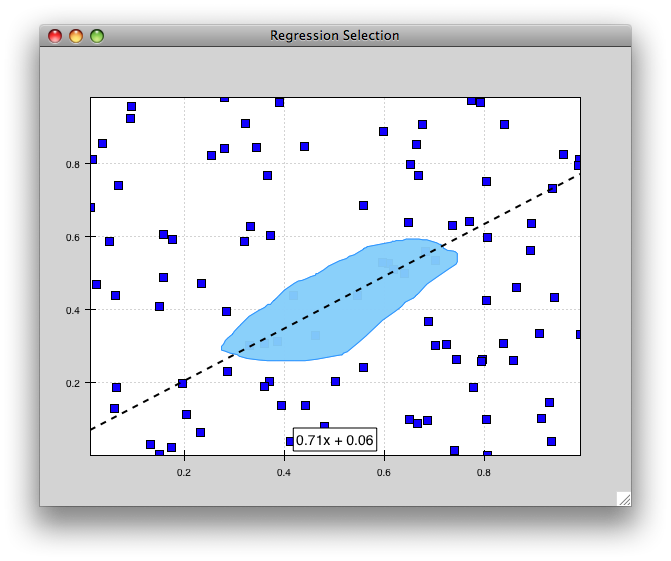
\includegraphics[height=2in, interpolate=true]{images/chaco_regr}
    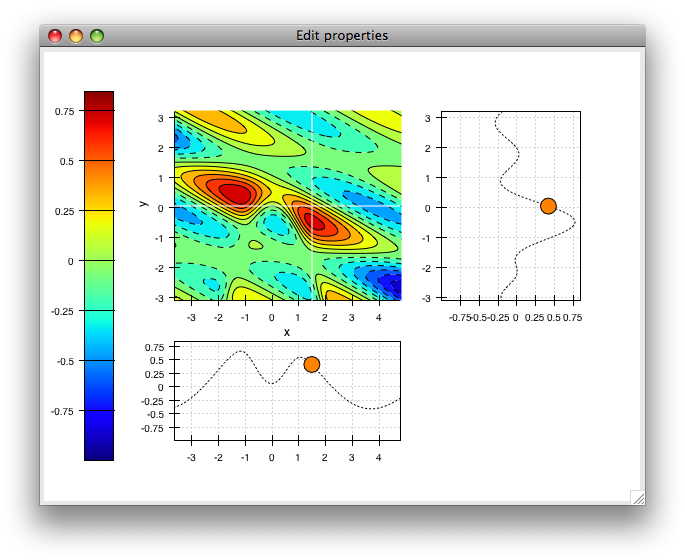
\includegraphics[height=2in, interpolate=true]{images/chaco_cmapi}
\end{center}
\end{frame}


\begin{frame}
  \frametitle{Chaco Architecture Overview}
  \begin{itemize}

      \item Data Handling: wrap input data, transform co-ordinates
          between data and screen space (eg., \typ{ArrayDataSource,
          LinearMapper})

      \item Visual components: render to the screen (eg. \typ{LinePlot,
          ScatterPlot, Legend, PlotAxis, ...})

      \item Tools: handle keyboard or mouse events and modify other
          components (eg. \typ{PanTool, ZoomTool, ScatterInspector})

  \end{itemize}
\end{frame}

\begin{frame}[fragile,plain]
\frametitle{Simple LinePlot}
\footnotesize
\begin{lstlisting}
class LinePlot(HasTraits):
    plot = Instance(Plot)
    traits_view = View(
        Item('plot',editor=ComponentEditor(), 
             show_label=False),
             width=500, height=500,
        resizable=True,
        title="Chaco Plot")

    def _plot_default (self):
        x = linspace(-14, 14, 100)
        y = sin(x) * x**3
        plotdata = ArrayPlotData(x = x, y = y)
        plot = Plot(plotdata)
        plot.plot(("x", "y"), type="line", color="blue")
        plot.title = "sin(x) * x^3"
        return plot
\end{lstlisting}
\end{frame}

%
%\begin{frame}[fragile,plain]
%\frametitle{Plotting the ODE Solution}
%\scriptsize
%The Plot view, plot and the old solution. ODE can be obtained from ODESolver,
%so it can be a property.
%XXX: tmpl
%\begin{lstlisting}
%class ODEPlot(HasTraits):
%    """ A 2D plot of ode solution variables. """
%    plot = Instance(Component)
%    # We need to set data when solution changes
%    pd = Instance(ArrayPlotData, args=())
%
%    ode = Property(Instance(ODE), depends_on='ode_soln')
%    ode_soln = Instance(ODESolver)
%    traits_view = View(Item('plot', editor=ComponentEditor(),
%                            show_label=False),
%                       resizable=True, title="ODE Solution")
%
%    def _get_ode(self):
%        return self.ode_soln and self.ode_soln.ode
%    ...
%    def _set_arr(self, name, key='index'):
%        if name == self.ode.t_var:
%            arr = self.ode_soln.t_arr
%        else:
%            arr = self.ode_soln.soln_arr[:, self.ode.vars.index(name)]
%        self.trait_set(**{key+'_arr':arr})
%
%    @on_trait_change('ode_soln.soln_arr')
%    def _on_soln_changed(self):
%        self.pd.set_data('index', self.ode_soln.t_arr)
%        self.pd.set_data('index', self.ode_soln.soln_arr[:, 0])
%
%    def _plot_default(self):
%        plot = Plot(self.pd)
%        plot.tools.append(TraitsTool(component=plot))
%        plot.tools.append(ZoomTool(component=plot))
%        plot.tools.append(PanTool(component=plot))
%        plot.plot(('index', 'value'))
%        return plot
%\end{lstlisting}
%\end{frame}


\begin{frame}[fragile,plain]
\frametitle{Plotting the ODE Solution}

The Plot view, plot and the old solution. ODE can be obtained from ODESolver,
so it can be a property.

\footnotesize
\begin{lstlisting}
class ODEPlot(HasTraits):
    """ A 2D plot of ode solution variables. """
    plot = Instance(Component)
    # We need to set data when solution changes
    pd = Instance(ArrayPlotData, args=())

    ode = Property(Instance(ODE), depends_on='ode_soln')
    ode_soln = Instance(ODESolver)

    def _get_ode(self):
        return self.ode_soln and self.ode_soln.ode
    ...
\end{lstlisting}
\end{frame}

\begin{frame}[fragile,plain]
\frametitle{Plotting the ODE Solution}
\footnotesize
We can create a plot using the first solution array.
\begin{lstlisting}
class ODEPlot(HasTraits):
    ...
    traits_view = View(
            Item('plot', editor=ComponentEditor(),
                 show_label=False),
            resizable=True, title="ODE Solution")

    def _plot_default(self):
        self.pd.set_data('index', self.ode_soln.t_arr)
        # Set the first array as value array for plot.
        self.pd.set_data('value', self.ode_soln.soln_arr[:,0])
        plot = Plot(self.pd)
        # Add some interactivity to the plots.
        plot.tools.append(TraitsTool(component=plot))
        plot.tools.append(ZoomTool(component=plot))
        plot.tools.append(PanTool(component=plot))
        plot.plot(('index', 'value'))
        return plot
\end{lstlisting}
\end{frame}

\begin{frame}[fragile,plain]
\frametitle{Plotting the ODE Solution}
We can make the plot react to changes to the solution
(changing initial condition etc.)
\footnotesize
\begin{lstlisting}
class ODEPlot(HasTraits):
    ...
    @on_trait_change('ode_soln.soln_arr')
    def _on_soln_changed(self):
        self.pd.set_data('index', 
                self.ode_soln.t_arr)
        self.pd.set_data('value', 
                self.ode_soln.soln_arr[:, 0])
\end{lstlisting}
\end{frame}

%%%%%%%%%%%%%%%%%%%%%%%%%%%%%%%%%%%%%%%%%%%%%%%%%%%%%%%%%%%%%%%%%%%%%%%%%%%%%%%
\section{Mayavi}

\begin{frame}
  \frametitle{Mayavi}
  \begin{itemize}
      \item \typ{from mayavi import mlab}
      \item Easy to use
      \item Uses Traits/TraitsUI heavily
      \item Can embed 3D plots
 \end{itemize}
\end{frame}

\begin{frame}[plain, fragile]
    \frametitle{A simple plot}
    \begin{columns}
        \column{0.5\textwidth}
        \myemph{\Large 1D data}

        \column{0.5\textwidth}
    \pgfimage[width=2in]{images/plot3d_ex}
    \end{columns}

    \begin{lstlisting}
>>> from numpy import *
>>> t = linspace(0, 2*pi, 50)
>>> u = cos(t)*pi
>>> x, y, z = sin(u), cos(u), sin(t)

    \end{lstlisting}

    \emphbar{\PythonCode{>>> mlab.plot3d(x, y, z, t)}}
\end{frame}


\begin{frame}[plain, fragile]
    \frametitle{Changing how things look}

    \begin{block}{Clearing the view}
    \typ{>>> mlab.clf()}
    \end{block}

    \pause

    \begin{block}{IPython is your friend!}
    \PythonCode{>>> mlab.points3d?}

    \begin{itemize}

        \item Extra argument: Scalars

        \item Keyword arguments

        \item UI
    \end{itemize}
    \end{block}
\end{frame}

\begin{frame}[fragile,plain]
\frametitle{Embedding a 3D plot}
\footnotesize
\begin{lstlisting}
from mayavi.core.ui.api import MayaviScene, \
    MlabSceneModel, SceneEditor

class Plot3D(HasTraits):
    scene = Instance(MlabSceneModel, args=())
    view = View(Item(name='scene',
                     editor=SceneEditor(
                         scene_class=MayaviScene),
                     show_label=False, resizable=True,
                     height=500, width=500),
                resizable=True)
\end{lstlisting}
\pause
\begin{lstlisting}
   @on_trait_change('scene.activated')
   def generate_data(self):
        # Create some data
        X, Y = mgrid[-2:2:100j, -2:2:100j]
        R = 10*sqrt(X**2 + Y**2)
        Z = sin(R)/R
        self.scene.mlab.surf(X,Y,Z,colormap='gist_earth')
\end{lstlisting}
\end{frame}

\begin{frame}[plain]
    \frametitle{Exercise}
\normalsize
  \begin{block}{Add a slider to the UI}
      Add a Range slider to the above example to change the
       \typ{R = 10*sqrt(X**2 + Y**2)} to 
       \typ{R = self.factor*sqrt(X**2 + Y**2)}
       such that the \typ{factor} can be adjusted.
  \end{block}
\end{frame}

\begin{frame}[fragile,plain]
\frametitle{Solution}
\footnotesize
\begin{lstlisting}
from traits.api import Range # <--
class Plot3D(HasTraits):
    scene = Instance(MlabSceneModel, args=())
    factor = Range(0.0, 20.0, 10.0) # <--
    view = View(Item(name='scene', 
                     # ...
                     ),
                Item(name='factor'), # <--
                resizable=True)

   @on_trait_change('scene.activated, factor') # <--
   def generate_data(self):
        # ...
\end{lstlisting}
\end{frame}

%%%%%%%%%%%%%%%%%%%%%%%%%%%%%%%%%%%%%%%%%%%%%%%%%%%%%%%%%%%%%%%%%%%%%%%%%%%%%%%
\section{Putting it all together}

\begin{frame}
  \frametitle{The application}
  \begin{itemize}
      \item Easy to put this together
      \item Exercise for you!
 \end{itemize}
\end{frame}

\begin{frame}
  \frametitle{So what?}
  \begin{itemize}
      \item Focus on the object model
      \item Solve the actual problem
      \item Model separation
      \item Easy to ``wire-up''
      \item UI is mostly declarative
 \end{itemize}
\end{frame}


\begin{frame}[plain]
  \frametitle{}
  \begin{center}
      What next?
  \end{center}
\end{frame}


%%%%%%%%%%%%%%%%%%%%%%%%%%%%%%%%%%%%%%%%%%%%%%%%%%%%%%%%%%%%%%%%%%%%%%%%%%%%%%%
\section{Note on Envisage}

\begin{frame}
  \frametitle{Envisage}
  \begin{itemize}
      \item Extensible framework
      \item \typ{Plugins}
      \item \typ{ExtensionPoints}
      \item \typ{Extensions}
      \item Similar to Eclipse
 \end{itemize}
\end{frame}

\begin{frame}[fragile]
  \frametitle{Application frameworks \ldots}
  \begin{block}{Central idea}
    \begin{itemize}
    \item Developer focuses on making a clean library
    \item Framework API specifies how different pieces of the app
      interact
    \item Plugin writer exposes the library or objects involved into
      the framework
    \item Application writer uses plugins to create new application
      easily
    \end{itemize}
  \end{block}
\end{frame}


\begin{frame}
  \frametitle{Application frameworks \ldots}
  \begin{center}
    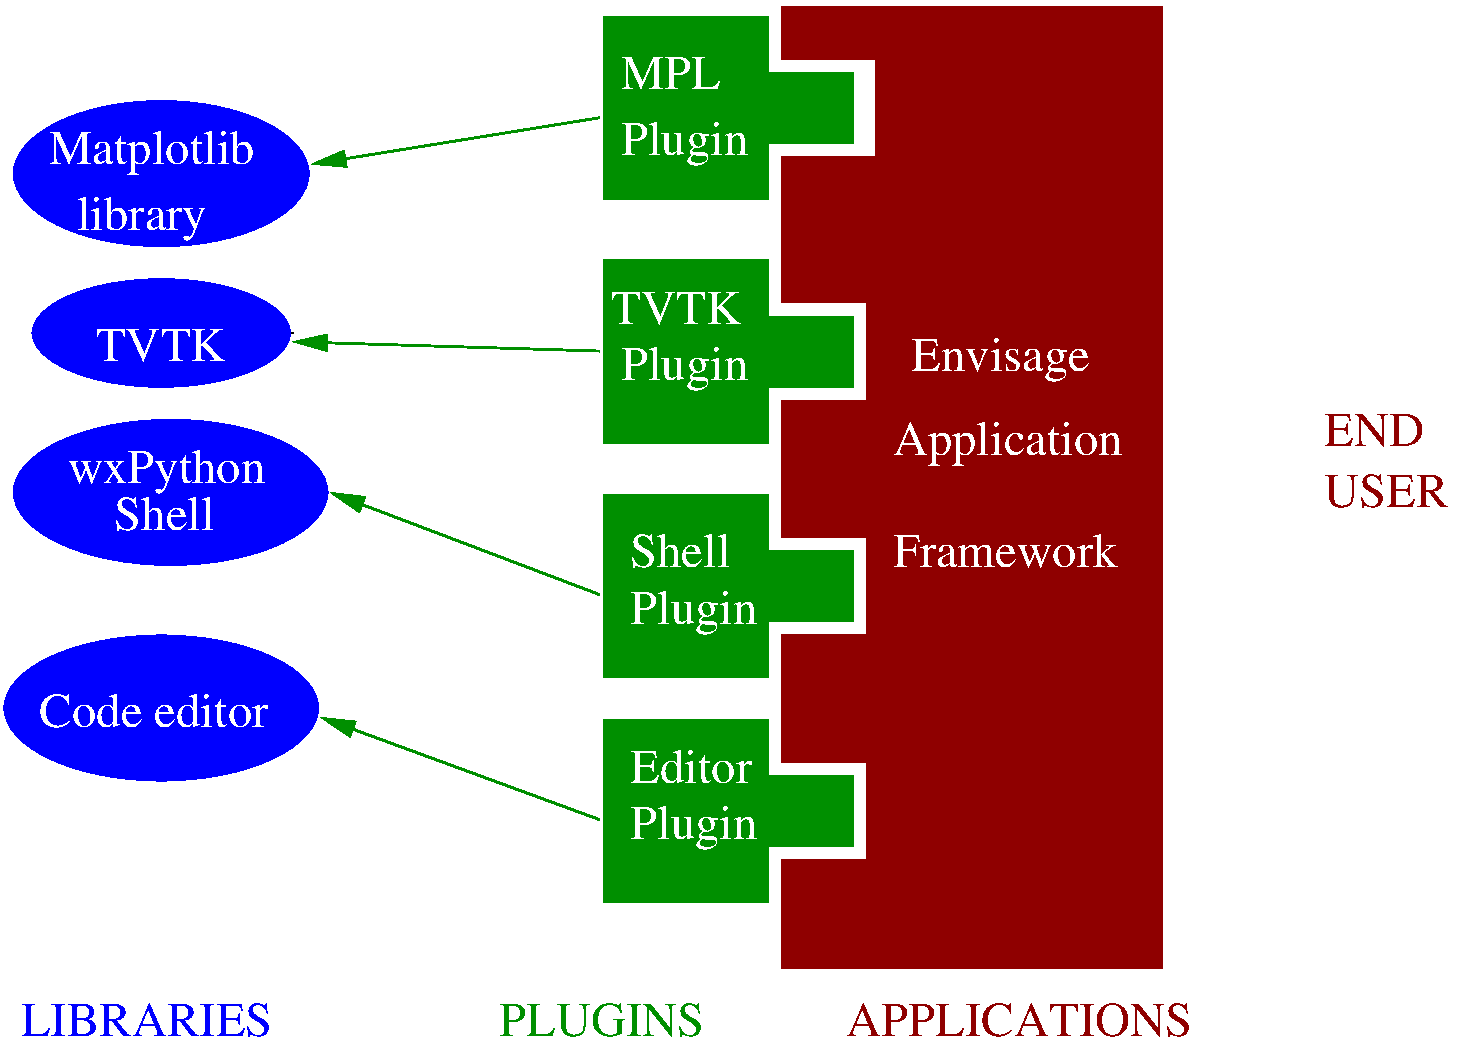
\includegraphics[width=3.75in,interpolate=true]{images/framework}
  \end{center}
\end{frame}


\begin{frame}
  \frametitle{Big picture}
  \begin{block}{Application and plugins}
    \begin{itemize}
    \item Envisage application: given a list of plugins
    \item Plugins setup their contributions
    \item Application starts: all plugins are started
    \item Plugins add their capabilties to the app
    \item Application stops: all plugins are stopped
    \end{itemize}
  \end{block}
\end{frame}

\begin{frame}
  \frametitle{Big picture}
  \begin{block}{Interaction/communication between plugins}
    \begin{itemize}
    \item Plugins define extension points
    \item Extensions $\rightarrow$ extension points
    \item Services
      \begin{itemize}
      \item Well known/shared objects
      \item Can be registered and looked-up with the application
      \end{itemize}
    \end{itemize}
  \end{block}
\end{frame}

\begin{frame}
  \frametitle{Envisage application}
  \begin{center}
    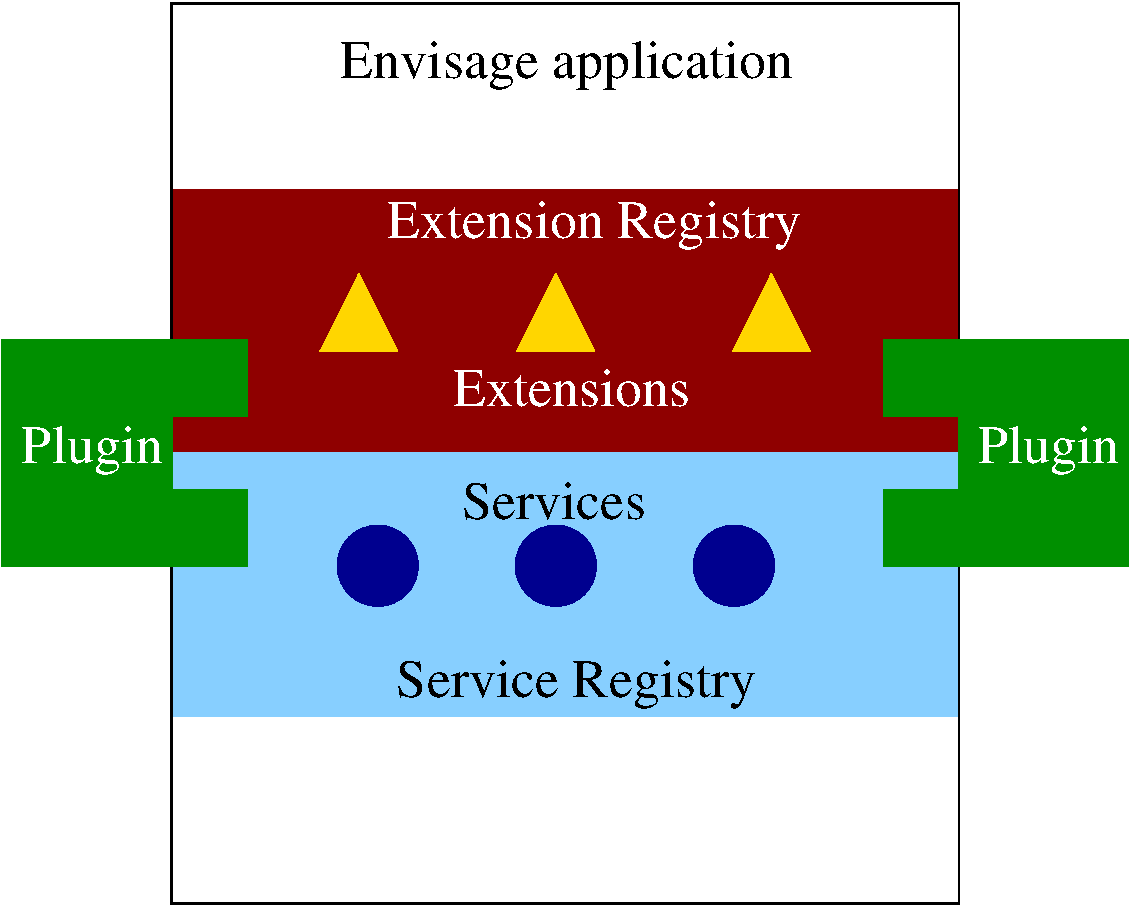
\includegraphics[width=3.5in,interpolate=true]{images/envisage}
  \end{center}
\end{frame}


\section{Summary}

\begin{frame}
  \frametitle{Summary}
  \begin{itemize}
      \item Traits
      \item TraitsUI
      \item Chaco
      \item Mayavi
      \item Envisage
 \end{itemize}
\end{frame}

\end{document}

%%%%%%%%%%%%%%%%%%%%%%%%%%%%%%%%%%%%%%%%%%%%%%%%%%%%%%%%%%%%%%%%%%%%%%%%%%%%%%%



